\documentclass[11pt]{article}
% RFP specifically says to use 11 point type and 1 inch margins
\usepackage{graphicx}
\usepackage{epsf,color}
\textwidth=6.5in\oddsidemargin=0in \evensidemargin=0in \topmargin
0pt \advance \topmargin by -\headheight \advance \topmargin by
-\headsep \textheight 9.0in

%\textwidth=6.5in\oddsidemargin=0in \evensidemargin=0in \topmargin
%0pt \advance \topmargin by -\headheight \advance \topmargin by
%-\headsep \textheight 8.9in

\usepackage{amsmath}
\usepackage{graphicx}
\usepackage{dcolumn}
\usepackage{multirow}
\usepackage{wrapfig}
\usepackage[compact]{titlesec}

%\usepackage[plain]{fullpage}
\usepackage{amsfonts}
%\usepackage{lastpage}
%\usepackage{fancyhdr}

%\usepackage[version=3]{mhchem} 
% you can use this command to skip chunks of your document
% just put the command around the chunk like this
% \comment{ ...the chunk... }
\newcommand{\comment}[1]{}

%\newcommand{\MarginPar}[1]{\hspace{1sp}\marginpar{\tiny\sffamily\raggedright\hspace{1sp}#1}}
\setlength{\marginparwidth}{0.75in}
\newcommand{\MarginPar}[1]{\marginpar{%
\vskip-\baselineskip %raise the marginpar a bit
\raggedright\tiny\sffamily
\hrule\smallskip{\color{red}#1}\par\smallskip\hrule}}

%\renewcommand{\baselinestretch}{1.05} % = 1.0 Single space; = 2.0 Double
\renewcommand{\baselinestretch}{1.0} % = 1.0 Single space; = 2.0 Double

%\renewcommand{\refname}{Literature Cited}
%------------------------

%\pagestyle{empty}  % No page numbers
%\textfloatsep 0mm
%\abovecaptionskip 1mm

\begin{document}

%\pagestyle{plain}
%\pagenumbering{roman}
\begin{center}
{\large{\textbf{A Hierarchical Approach to Uncertainty Quantification}}}

\vskip\baselineskip
{\large{ Lead PI:  J. Bell \\
Senior/Key Personnel: M. Day, J. Goodman, P. Graf, R. Grout, M. Morzfeld, G. Pau}}
\end{center}

\subsection*{Background}

Many important DOE applications rely on simulation to predict the behavior of complex physical systems.
%\MarginPar{wanted to maintain homage to exascale}
However, the fidelity of these simulations depends on uncertain parameters describing the underlying physical system
obtained from 
complex and noisy experiments whose reliability is hard to determine. 
Our ability to effectively use extreme scale computing will depend critically on our ability to reduce the
uncertainty in this data and assess the impact of that uncertainty on predictive capability.
Here, we will focus on combustion modeling, battery simulation and design of high-efficiency photovoltaic
devices as motivating examples; however, the methodology will be broadly applicable to a
range of problems in chemical and materials science, systems biology, subsurface flow and climate to name a
few.
%Most simulations that are important for DOE applications rely on parameters and models that are
%inferred from experiments.
%Complex and noisy experiments lead to parameter estimates whose reliability is hard to determine. 
%We propose to address these issues using a combination of novel simulation and sampling methods.
%We will focus on three applications: combustion modeling, battery simulation, and high-efficiency 
%photovoltaic devices.
%The methodology should be broadly applicable to a range of problems in chemical and materials 
%science, systems biology, subsurface flow, climate and other areas.

%({\em Not quite sure what this was getting at, so the following may be inaccurate.})

%To address the uncertainty in these types of problems we can no longer treat
%simulation and parameter estimation as separate activities.
For the class of problems we are targeting, there is typically a 
hierarchy
of experiments of increasing complexity that provide information about the underlying processes.
Rather than attempt to estimate parameters directly from a single complex experiment, we 
%\MarginPar{wanted to have more of a spanning across a hierarchy of data of increasing complexity}
will obtain parameter estimates across the entire hierarchy of experiments.
As experimental complexity increases the fraction of the state that can be sampled
by measurement is reduced and the cost of simulations increases; requiring that we pass
information through the hierarchy in a way that allows us to effectively use data from all levels
to improve overall predictive properties.
Furthermore, as complexity increases,
the combination of rich physics and relative data sparsity suggests that we will not be
able to exactly match the experimental dynamics computationally.
We must develop estimation methods that are robust to model errors as well as noisy observations
using metrics based on identification of characteristic features that are more general than
traditional quantities of interest.

The goal of this project is to develop a
mathematical framework for this class of problems that will allow us to (1) use available data from a hierarchy
of experiments of increasing scale and complexity to restrict
uncertainty in the description of the system, (2) estimate the impact of the improved characterization
on predictive capability and (3) identify which of the remaining uncertainties have the most impact
on the uncertainty of predictions.
We propose to address these issues using a combination of novel simulation and sampling methods that
intertwine parameter estimation and simulation into an integrated activity.
%\emph{Moreover, the UQ tools that we will produce based on our general framework will be designed to be efficient on future computer architectures.}


\subsection*{Approach}
We propose a Bayesian UQ framework based on Monte Carlo (MC) sampling.
The Bayesian approach avoids the need for additional approximations and simplifying assumptions 
required by some current UQ techniques.
It combines modeling and sampling in a way that provides full insight into the propagation of 
uncertainty.
The posterior distribution contains all information about remaining uncertainties that is implied
by the data -- which aspects are tightly bounded and which are less precise.
In addition, some MC sampling methods are well suited to massively parallel computer architectures because
the computationally expensive calculations
(e.g. forward or adjoint model runs) can be executed independently.
Using MC sampling as the computational backbone will lead to a numerically sound implementation of a rigorous UQ theory
that is well suited for future (exascale) machines, making UQ possible for realistic applications.

%A core problem with current MC techniques is that they rely on prior sampling, which is problematic because,
%from a Bayesian perspective, high-probability events with respect to the prior are likely to have low
%probability with respect to the posterior. In short, the scaling of the number of prior samples with the number
%of dimensions of the problem is so poor that MC sampling is infeasible even for moderate scale problems;
%it is expected that large scale applications are still out of reach even when the number of samples can be
%increased dramatically by extreme-scale computing.
The key issue with a Bayesian UQ approach is that current sampling techniques
are not robustly effective for complex, high-dimensional problems.
Standard particle filter methods break down in high dimensions because high-probability events 
with respect to the prior are likely to have low probability with respect to the posterior. 
Metropolis and heat bath algorithms suffer on problems that are poorly conditioned.
One of the central themes of this project will be to develop new smart sampling technologies 
to address these issues.
One possibility here is the implicit sampling methodology developed at LBNL.
The central idea is to avoid prior sampling by finding a probability distribution that approximates the
relationship between parameters and data; the search for a suitable approximate distribution is implemented
via solution of a minimization problem.
When available we can use adjoint codes coupled to BFGS-type algorithms to solve the minimization problem
using a parallel optimizer such as TAO from Argonne.
%\MarginPar{JG doubts this will work and notes a need to for derivative information to guide sampling. JBB
%doubts we can perform adjoint simulations for 3 turbulent simulations.  Only way out JB can think of
%is based on discussion with George about combining coarse simulation with a statistical surrogate to
%build an estimate of finer response . . . Unless someone has a brilliant idea here i suggest we leave this
%for the preproposal and thing of how to address it in real proposal}
However, when adjoint codes are unavailable, derivative free optimization methods will be required.
The most interesting and likely most successful type of approach here is a surrogate method,
where a small number of forward simulations are utilized to generate a simplified model of the simulation.
This model is then used in the optimization and its further refinement goes hand in hand with its use
in seeking the minimum.
Many research questions surround the interplay between optimization and
and sampling, particularly with approximate surrogate models.

Another key problem that has to be addressed for effective sampling is dealing with model degeneracy.
A model has an approximate degeneracy if many different parameter sets are nearly as good at explaining the data.
For example, if there are multiple reaction pathways in a kinetic description,
certain combinations of reaction rates may be much better
estimated than the individual rates.
In such cases, isotropic sampling algorithms such as single variable heat bath (Gibbs sampler) or isotropic
Metropolis walk will be slow. We plan to use the affine sampling approaches developed at NYU to address issues of model degeneracy.

Finally, it is important to use statistical methods that are robust in the inevitable situation where the exact model is not in
the family being fit.
For example, the power law/exponential formulas for reaction rates are only modeling approximations, though they can be
very accurate.
In chaotic systems especially, even small modeling errors can make an accurate global fit impossible.
One approach is to include noise in the dynamics, so that the posterior distribution does not require the
dynamical equations to be satisfied exactly.
We will conduct computational experiments to study this problem, then use the results to 
choose appropriate noise levels for our physical models.
By combining what is known about the error levels in both model and data, we can also estimate upper and lower bounds
of the predictive skills of the resulting stochastic models.

As noted above, reduced order models can be used to construct surrogates as part of a derivative free optimization strategy
to guide the sampling procedure. However, our goal is to also use reduced order models for an {\it {a posteriori}} UQ analysis.
For this purpose, the selection of an appropriate reduced order model at each level of the hierarchy depends on the
structure of the system at this level, ranging from model reduction approaches for models with smooth solution manifolds
to statistical approaches for complex models.
Given a hierarchy of reduced order models, this proposal will address how we can perform an integrated UQ analysis 
across the hierarchy, taking into accounts different levels of scale and fidelity.
%Given an appropriate reduced order model, after we have completed a suite of samples across the hierarchy
%we can then use the reduced order models to perform an uncertainty quantification analysis across
%the hierarchy.  
This analysis not only defines the predictive capability of the models, it also identifies
the major factors contributing to uncertainty and identifies what additional data would most significantly
impact the fidelity of predictions.

To evaluate the methodology we will examine test cases within each of our target application areas.  In particular,
we will consider thermodiffusive instabilities in turbulent hydrogen flames, robustness of Li-ion batteries under abusive conditions
and the formation of point defects in new photovoltaic materials.  In each case, we will focus on how uncertainties in the 
model parameters influence predictive capability and how we can reduce uncertainty using a hierarchy of experimental data.
\end{document}
%NEED SOMETHING ABOUT ROLE OF REDUCED ORDER MODELS.  I THINK ONE USE OF REDUCED ORDER
%MODELING IS TO GUIDE THE SMART SAMPLING APPROACHES IN MONTE CARLO.  ALSO SHOULD BE
%USEFUL IN SCALE BRIDGING BUT THAT IS MORE TENUOUS IN MY HEAD.

Examples:

\subsection*{Turbulence/Chemistry Interaction example:}

Inputs: Chemical kinetics and transport parameters with initial priors
 
Hierarchical data sources (experiments): 0d ignition, 1d laminar flames, shock-tube experiments
2D laminar flame DNS, 3D turbulent flames

Objectives:
\begin{itemize}
\item Use available data to reduce uncertainty in kinetics and transport
\item Estimate the impact of the improved characterization on predictive capability for turbulent flames
\item Identify which of the remaining uncertainties have the most impact on the uncertainty of the predictions
\end{itemize}
 
\subsection*{Point defect formation in thin-film photovoltaics:}
A key design need for high efficiency photovoltaic devices, e.g. those
based on CZTS absorbers, is the ability to control the carrier
concentration to achieve n+ and p+ doping resulting from point
defects. The creation of the various types of defects (intrinsic ionic
and electronic defects) can be described by a set of kinetic reaction
equations. For example, an abstract metal-sulfide system could be
described by simplistic system expressing an oxidation reaction, the
Schottky disorder and creation of anion vacancies:

\ce{ \tfrac{1}{2} S2 -> S_s^x + V_m^{''} + 2 h^+ }

\ce{ NULL -> V_m^{''}+ V_s^{$\cdot \cdot$} }

\ce{ NULL -> e^' + h^{$\cdot$} }

\ce{ S_s^x -> \tfrac{1}{2} S2 + V_s^{$\cdot \cdot$} + 2 e^- }

Near first-principles calculations such as electronic structure
calculations based on density functional theory can provide enthalpy
differences for the formation of these various point defects.
Neglecting the entropic contribution to the Gibbs energy, this
information is sufficient to determine equilibrium concentrations that
can be used to coarsely estimate the variation of the material
characteristics with the key parameters. For the system above, the
$S_2$ partial pressure is a key variable that when varied leads to a
Kroger-Vink diagram with the classic form shown in Figure~\ref{fig:kv}
where the crossover point between electron/hole concentrations is at
the stoichiometric pressure. \begin{figure}[h!]
  \centering
  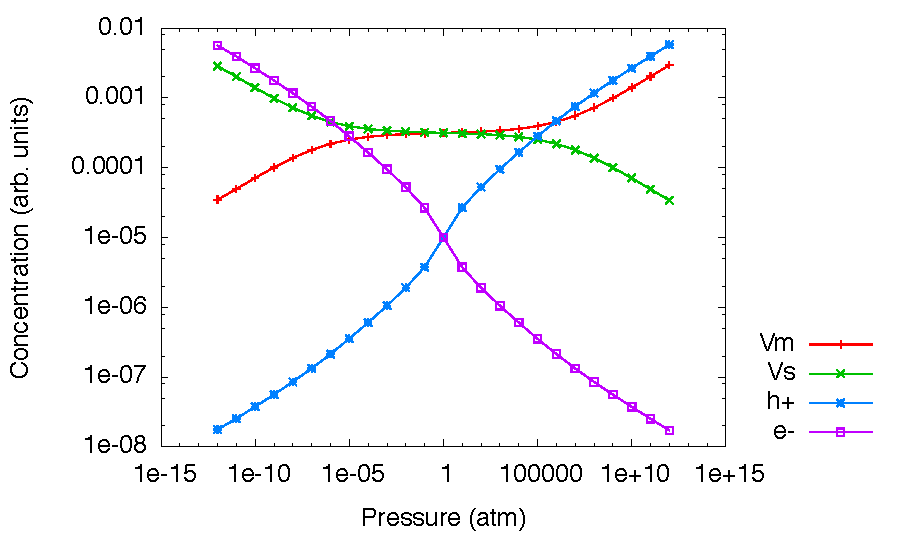
\includegraphics[width=0.8\textwidth]{KV.pdf}
  \caption{Kroger-Vink diagram for generic M-S system}
  \label{fig:kv}
\end{figure}
Even for this simplistic system, time-varying histories of the
non-metal pressure and temperature during crystal growth can be
expected to access quasi-equilibrium states. Additional parameters in
the Arrhenius forms for the kinetic rate expressions are required to
determine a time-dependent solution capable of predicting these states
with associated uncertainty. Complicating measurements that can be
used to estimate these parameters, diffusion of the non-metal species
($S_2$ above) into the film may be rate-limiting. Further, measurement
of the concentration of arbitrary point defects is difficult and must
be inferred from more easily observed characteristics. For realistic
systems, involving 10s to 100s of such kinetic expressions, many such
states with desirable properties may exist. Such states may be of
interest in two forms: firstly, they may useful for design of PV
systems, and secondly, they may have measurable characteristics that
allow us to reduce the uncertainty associated with one or more rates,
thereby allowing other states to be found that are useful for actual
devices.

In contrast to well-studied combustion chemical kinetics, where a
relatively (if still insufficient) quantity of experimental data points
have been acquired ti validate reaction mechanisms, point-defect systems are relatively poorly
understood. Many more experiments are necessary to converge on a
reasonable representation of the appropriate rates. 


FLESH OUT FROM RAY'S NOTES

\subsection*{Missing issues / concerns}

\begin{enumerate}
\item Need to flesh out more examples
\item How should we address the extreme-scale computing aspects of this
\item Fix general flakiness and flesh out places where help is needed
\end{enumerate}

\newpage

\section*{Matti's raw notes}


\begin{itemize}
\item Essentially all problems are non-linear and exhibit non-Gaussian statistics and, therefore, Monte Carlo sampling will be at the core of modern and next generation UQ techniques
\item Monte Carlo sampling is well suited for parallel computer architectures because the computationally expensive calculations (e.g. forward or adjoint/backward model runs) can be executed independently; the necessary communication happens only via scalar quantities, so that very little data must be moved across nodes
\item Due to a catastrophic scaling of the number of Monte Carlo simulations required with the number of dimensions of the underlying probability space, brute force Monte Carlo is not feasible for large-scale problems, even on exascale machines
\item New sampling techniques, developed at LBNL have shown promise in UQ in engineering problems (O(10) dimensions, e.g. in robotics, tracking of satellites) and in small scale geophysical inverse problems  (and their UQ, O(500) dimensions). The geophysical inverse problems are large enough such that traditional Monte Carlo is hopeless (on current and future machines).
\item We have experience with new sampling techniques for UQ, inverse problems and target tracking
\item The "technology" is ready for the next step: explore applicability to large/extreme scale problems, in particular (i) use of extreme scale minimization techniques (derivative free minimization, adjoint calculations, limited memory quasi-Newton methods); (ii) minimizing communication between cores/nodes and data movement/storage during sampling and updating; (iii) integration with large (extreme) scale simulation codes; (iv) a study of the scaling of the algorithm with the number of cores
\item Result: first large scale UQ system with smart Monte Carlo sampling and without Gaussianity or linearity assumptions
\item UQ  capabilities: UQ without Gaussianity or linearity assumptions; integration of experimental data and mathematical model/numerical codes; accurate tracking of uncertainty (e.g. covariances of errors); forecasting under uncertainty.

\end{itemize}


\section*{Ray's raw notes}

Thematic elements:

Manifold discovery / slow attractors

Link input parameters to changes in slow attractor

Identify observables based on characteristics of slow attractor that are related to changes in input parameters, specifically those we wish to investigate

Design framework so that each experiment conducted narrows the distribution of the priors to provide a strong probability of finding a change in attractors or measurable difference in output. 

Searching for transformation between distribution of inputs and distribution of outputs. 

Quantify the utility of an experiment by the degree of reduction in uncertainty

Use guided search based on priors to restrict the search space

Turbulence/Chemistry Interaction example:


Inputs: Chemical kinetics parameters, geometry, initial conditions

Traditional outputs: net overall burning rate in turbulent flame at device conditions

Candidates for optimal observable: reaction rate of each of n species, creation/destruction rates, vector indicating participation in each possible reaction pathway, vector indicating species participation.
(These are based on physical insight -- is it necessary to presuppose the candidates for observables?)
 
Data sources (experiments) hierarchy: 0d ignition simulation, 1d laminar flame simulation, library of 1d laminar flame experiments at conditions that perturb expected chemistry, ODT based laminar flame solution, 2D turbulent flame DNS, 3D turbulent flame DNS, shock tube ignition delay time parametric study.

Objective: Determine which chemical kinetics parameters to study further; design experiments with appropriate observables to objectively compare different kinetic mechanisms; design experiments to assess the impact of changing fuels (and hence mechanisms).

Point defect formation application:
Inputs: Potential kinetic mechanism; estimated activation energies based on DFT calculations; process conditions:

Observables: Quasi-equilibrium concentration of electrons in conduction band. 

Candidates for optimal observable: Individual point defect concentrations. 

Experimental hierarchy: Deterministic calculation of 0D equilibrium state, parametric in environmental conditions; experimental film growth with parametric variation of surface pressure, T (shifts relative rate of reactions); film growth in light/dark (may enable/disable defect formation mechanism); deterministic computation coupled to 1D transport; stochastic sampling of defect formation rates (using kinetic rates as transition probabilities).

Outcome: Determine process conditions that increase the probability of a favorable point defect configuration. Find the metastable states /attractors; assess these for favorable properties; engineer process likely to produce them. 

Other application areas:
\begin{itemize}
\item Anything with a reaction/kinetic network with uncertain parameters
\item Quantifying ``usefulness'' of expensive experiments
\item Kinetics of biological biomass deconstruction
\item Cosmology
\item OPV degradation rate modeling
\item Groundwater decontamination modelling 
\end{itemize}

Requisite features of application area:
\begin{itemize}
\item Model that can relate input parameters to observables with a hierarchy of fidelity
\item Targeted for kinetic reaction networks (conceivably this could be relaxed)
\item Dynamic / chaotic system with an underlying attractive manifold 
\item Finite number of attractors that can be described by continuous characteristics
\end{itemize}


%\newpage

\bibliographystyle{plain}

\bibliography{george_rom.bib} 



\end{document}
